% Select T1 before IEEEtran initializes Times, including with XeTeX/Tectonic.
\RequirePackage[T1]{fontenc}
\documentclass[journal]{IEEEtran}

% GRSL submission manuscript: IEEE journal format, 10 pt, two columns.
\usepackage{amsmath,amssymb,bm}
\usepackage{booktabs}
\usepackage{tabularx}
\usepackage{array}
\usepackage{graphicx}
% Enable bottom placement of double-column floats without changing spacing.
\usepackage{stfloats}
\usepackage{cite}
\usepackage{url}

\newcommand{\vect}[1]{\bm{#1}}

% Original comparison images, placed without resampling; labels remain 8 pt.
\newcommand{\comparisonpanel}[3]{%
  \begin{minipage}[t]{0.24\columnwidth}
    \centering
    \includegraphics[width=\linewidth]{#1}\par
    \vspace{2pt}%
    {\footnotesize\strut #2\par\strut #3\par}
  \end{minipage}%
}

\begin{document}

\title{SAR Despeckling via Fourier Refinement and
Representation-Consistent Reconstruction}

\author{Hongyu~Chen, Peng~Liu,~\IEEEmembership{Senior~Member,~IEEE}%
\thanks{\raggedright\emph{(Corresponding author: Peng Liu.)}\par
The authors are with the Key Laboratory of Information Science of Electromagnetic Waves, Fudan University, Shanghai, China (e-mail: \mbox{pliu@fudan.edu.cn}).}}

\maketitle

\begin{abstract}
The discrepancy between simulated speckle and real synthetic aperture radar (SAR) observations limits the generalization of supervised despeckling models. We extend the public Trans-SAR backbone by incorporating full-spectrum Fourier-domain refinement and representation-consistent reconstruction. Specifically, one bottleneck block and five decoder blocks combine local features with real--imaginary channel mixing, and bounded log-intensity predictions are inverted before intensity compensation. Masked adaptation updates the reconstruction on noisy real SAR image while the Transformer encoder remains frozen. Across 8,400 simulated pairs from 21 UCMerced classes and four look numbers, the proposed model achieves macro-averaged peak signal-to-noise ratio (PSNR) and structural similarity index (SSIM) values of 28.14~dB and 0.7791, respectively, without requiring the number of looks as input. PSNR is highest among evaluated methods at every look. Removing the Fourier refinement reduces PSNR by 1.68~dB. On 592 patches from held-out parent images, adaptation lowers the M-index from 1.8213 to 1.3365 and improves the edge-preservation index from 0.4229 to 0.8214. These results validate the proposed reconstruction design and adaptation strategy on the evaluated datasets.
\end{abstract}

\begin{IEEEkeywords}
Synthetic aperture radar, despeckling, Transformer, Fourier refinement, self-supervised adaptation.
\end{IEEEkeywords}

\section{Introduction}
In synthetic aperture radar (SAR), speckle obscures edges, texture, and bright scatterers. Despeckling must recover these structures despite signal-dependent noise and the scarcity of clean references~\cite{fracastoro2021overview}. Although unit-mean Gamma corruption supports controlled multilook experiments, focused SAR image also contains spatially correlated speckle and processing artifacts. Consequently, restoration models trained on simulated pairs often generalize poorly to real-world observations.

Lee filtering uses local statistics~\cite{lee1980}, whereas SAR-BM3D exploits nonlocal recurrence and transform-domain shrinkage~\cite{parrilli2012}. Supervised CNNs learn paired restoration priors~\cite{chierchia2017}, with SAR-CAM adding continuous multiscale attention~\cite{ko2022}. Trans-SAR combines a hierarchical Transformer encoder with convolutional reconstruction~\cite{perera2022}; subsequent models introduce dynamic gates and noise-guided multiscale fusion~\cite{shen2025,zhang2025}. Frequency decomposition in SAR-FDD and DATNet complements spatial processing~\cite{shen2025,zhao2024}, while transformed conditional diffusion offers another representation for multiplicative statistics~\cite{ma2024}. However, speckle and scene structure overlap in the frequency domain, motivating joint local and spectral refinement that avoids predefined frequency bands.

The effectiveness of learning from real observations also depends on the type of supervision. SAR2SAR exploits multitemporal acquisitions~\cite{dalsasso2021}; Speckle2Void combines blind-spot likelihood training with decorrelation~\cite{molini2022}; and Speckle2Self uses masked self-supervision with attention~\cite{lin2025}. SDS-SAR constructs intensity-only training pairs through correlation-aware sampling~\cite{chen2026}, whereas SDUDNet employs unpaired clean and noisy images~\cite{bo2025}. These approaches motivate adaptation without clean targets, however, their differing assumptions require additional care when comparing restoration outcomes.

We extend the publicly available Trans-SAR backbone in three complementary directions. Specifically, six Fourier-domain refinement (FDR) blocks combine local filtering with full-spectrum real--imaginary channel mixing at the bottleneck and five decoder scales. Second, an exact inverse maps bounded log predictions back to intensity before residual compensation, keeping output fusion within one representation. Third, encoder-frozen masked post-adaptation (AMS) calibrates the reconstruction to real SAR image without requiring clean targets. \mbox{Fig.~\ref{fig:overview}} distinguishes the inherited operators from the additions. Controlled ablations assess the reconstruction components, while evaluation employs a single model across four look numbers plus a real-SAR split with disjoint parent images. The real-data evidence is empirical, indicating that masked noisy targets do not guarantee unbiased restoration under correlated speckle.

% Scope retained: explicit Trans-SAR inheritance; actual six-block layout;
% exact inverse only applies to the bounded log transform; no look-number input;
% parent-disjoint real evaluation; no clean-target or unbiasedness claim.
% All 15 literature keys cited by the original Introduction/Related Work remain.

\begin{figure*}[!t]
  \centering
  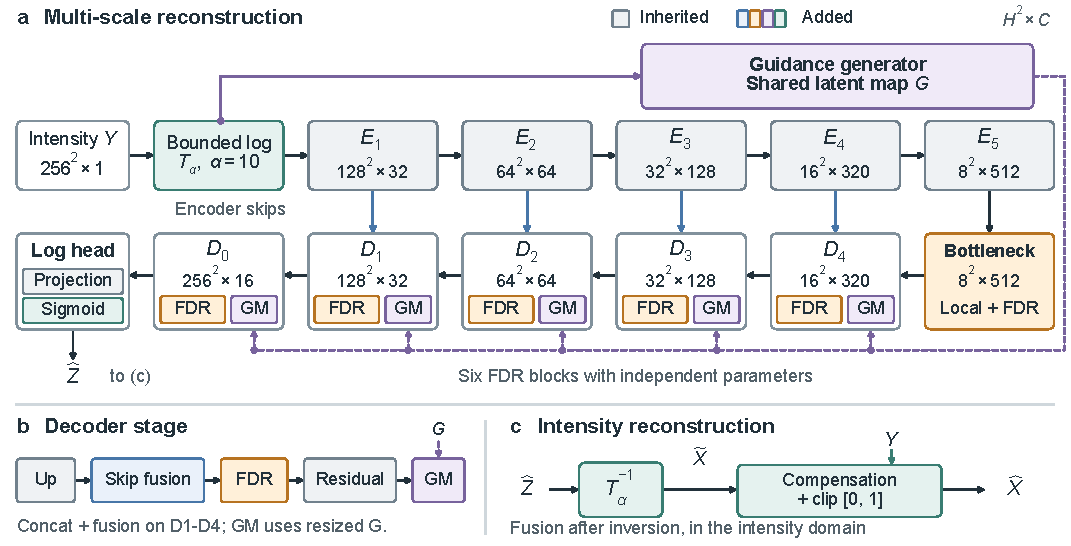
\includegraphics[width=\textwidth]{figures/fig1_overall_architecture.pdf}
  \caption{(a) Encoder--decoder overview; tensor labels give spatial size $\times$ channels. Gray marks inherited operators, and colors mark additions. Six FDR blocks have independent parameters. (b) Decoder order: skips concatenate encoder features before fusion; $D_0$ has no skip. GM denotes stage-specific guidance modulation using the resized shared map $G$. (c) Log predictions are inverted before intensity compensation with original $Y$ and clipping.}
  \label{fig:overview}
\end{figure*}

\section{Proposed Method}
\subsection{Observation and Reconstruction Path}
Let \(\vect{X},\vect{Y}\in[0,1]^{H\times W}\) denote a clean intensity proxy and its noisy observation. Synthetic pairs use independent Gamma speckle~\cite{perera2022} with look number \(L\). We clip the simulated intensities to \([0,1]\):
\begin{equation}
\begin{aligned}
\vect{Y} &= \operatorname{clip}(\vect{X}\odot\vect{N},0,1),\\
N_{ij} &\sim \operatorname{Gamma}(L,L^{-1}).
\end{aligned}
\label{eq:observation}
\end{equation}
The shape--scale parameterization gives unit mean and variance \(L^{-1}\) before clipping. This controlled corruption does not reproduce the full statistics of focused SAR image. We use the normalized logarithmic mapping in~\eqref{eq:log} and its algebraic inverse in~\eqref{eq:inverse}:
\begin{equation}
T_{\alpha}(\vect{Y})=
\frac{\log(1+\alpha\vect{Y})}{\log(1+\alpha)},
\qquad \alpha=10,
\label{eq:log}
\end{equation}
\begin{equation}
T_{\alpha}^{-1}(\widehat{\vect{Z}})=
\frac{\exp[\widehat{\vect{Z}}\log(1+\alpha)]-1}{\alpha}.
\label{eq:inverse}
\end{equation}
The mapping moderates bright intensities without assuming additive Gaussian noise in the transformed domain.

The encoder and basic upsampling operators follow Trans-SAR, including overlap embeddings and attention with spatial reduction~\cite{perera2022}. Its five stages have widths (32, 64, 128, 320, 512), head counts (1, 1, 2, 4, 8), and depths (3, 3, 4, 6, 3), with resolutions from \(128^2\) to \(8^2\). Reconstruction applies bottleneck refinement followed by five decoder stages, each ordered as upsampling, available skip fusion, FDR, residual convolution, and guidance modulation. A sigmoid head predicts bounded log intensity, which is inverted before intensity compensation.

\subsection{Fourier Refinement and Guided Compensation}
For feature \(\vect{F}\), FDR runs a spatial branch (depthwise \(3\times3\), pointwise projection, and Gaussian error linear unit (GELU) alongside an orthonormal two-dimensional real fast Fourier transform (FFT):
\begin{equation}
\begin{aligned}
\vect{Q} &= \operatorname{rFFT2}(\vect{F}),\\
\vect{Q}_{c} &= [\operatorname{Re}(\vect{Q}),
                   \operatorname{Im}(\vect{Q})].
\end{aligned}
\label{eq:fft}
\end{equation}
The real--imaginary concatenation follows the Fourier-unit representation in~\cite{chi2020ffc}. In our implementation, two real-valued \(1\times1\) convolutions separated by GELU mix the concatenated real--imaginary channels. Their weights are shared across frequency coordinates; neighboring frequencies are not convolved. Splitting the output and applying the inverse real FFT yields \(\vect{F}_{f}\), which our FDR module fuses with the spatial feature \(\vect{F}_{s}\):
\begin{equation}
\begin{aligned}
\vect{U} &= \operatorname{GELU}
 \bigl(\vect{W}_{o,1} * [\vect{F}_{s},\vect{F}_{f}]\bigr),\\
\operatorname{FDR}(\vect{F})
 &= \vect{F}+\vect{W}_{o,2}*\vect{U}.
\end{aligned}
\label{eq:fdr}
\end{equation}
where \(\vect{W}_{o,1}\) and \(\vect{W}_{o,2}\) are \(1\times1\) and \(3\times3\) convolutions, respectively. FDR processes the full spectrum without explicit bands or complex-valued convolution. Six independent blocks act at the bottleneck and decoder resolutions \(16^2\) through \(256^2\). The bottleneck also sums the FDR output with a local feature, projects the sum, and adds it to the input through a learnable scale initialized to 0.1.

A shared guidance branch jointly learns a single-channel latent map from the log input, without separate noise-map or look-number supervision. At each decoder scale, the resized map is concatenated with the feature; pointwise and \(3\times3\) convolutions produce \(\tanh\) modulation with a learnable scale initialized to 0.1. For the sigmoid prediction \(\widehat{\vect{Z}}\), let \(\widetilde{\vect{X}}=T_{\alpha}^{-1}(\widehat{\vect{Z}})\). Our model applies intensity compensation as
\begin{equation}
\begin{aligned}
\vect{R}_{c} &= F_{\mathrm{comp}}
 ([\vect{Y},\widetilde{\vect{X}}]),\\
\widehat{\vect{X}} &= \operatorname{clip}
 (\widetilde{\vect{X}}+\gamma_c\vect{R}_{c},0,1).
\end{aligned}
\label{eq:compensation}
\end{equation}
The compensator has two \(3\times3\), 32-channel GELU layers and a single-channel residual head. Its learnable \(\gamma_c\) starts at 0.1 without bounding the correction; final clipping constrains intensity. Both summands in~\eqref{eq:compensation} are in the same intensity representation.

\subsection{Supervision and Masked Adaptation}
Following the use of squared-error and total variation (TV) losses in~\cite{perera2022}, we adopt the following mean-normalized objective:
\begin{equation}
\mathcal{L}_{\mathrm{sup}}=
\frac{1}{HW}\lVert\widehat{\vect{X}}-\vect{X}\rVert_2^2
+\lambda_{\mathrm{TV}}^{\mathrm{sup}}\operatorname{TV}(\widehat{\vect{X}}).
\label{eq:supervised}
\end{equation}
TV is the sum of the mean absolute horizontal and vertical neighbor differences. Both TV weights are selected on their corresponding validation splits as described in Section~III-B. Following masked self-supervision~\cite{lin2025}, our AMS implementation masks pixels independently with probability 0.2 and uses their original noisy values as targets for masked L1 loss with TV on the full prediction:
\begin{equation}
\begin{gathered}
\vect{Y}_m=\vect{Y}\odot(1-\vect{M}),\qquad
\widehat{\vect{X}}_m=f_{\theta}(\vect{Y}_m),\\[3pt]
\mathcal{L}_{\mathrm{AMS}}=
\frac{\lVert\vect{M}\odot(\widehat{\vect{X}}_m-\vect{Y})\rVert_1}
{\max(\lVert\vect{M}\rVert_1,1)}
+\lambda_{\mathrm{AMS}}\operatorname{TV}(\widehat{\vect{X}}_m).
\end{gathered}
\label{eq:ams}
\end{equation}
Here, the network outputs intensity, and ones in the mask identify masked pixels. Only the Transformer encoder is frozen; the bottleneck, decoder, guidance, head, and compensator adapt for eight epochs at learning rate \(10^{-6}\). Training masks are resampled, whereas fixed validation masks support checkpoint selection at identical locations. Inference uses unmasked observations. During AMS, \(\vect{Y}_m\) replaces \(\vect{Y}\) throughout the network, including the compensator.

\begin{table*}[!b]
\caption{UCM-21 Gamma-Speckle Results on 8,400 Fixed Pairs}
\label{tab:main}
\centering
\footnotesize
\setlength{\tabcolsep}{3.2pt}
\renewcommand{\arraystretch}{1.08}
\begin{tabular*}{0.86\textwidth}{@{\extracolsep{\fill}}llccccc@{}}
\toprule
\textbf{Method} & \textbf{Look mode} &
\shortstack{\(L=1\)\\PSNR / SSIM} &
\shortstack{\(L=2\)\\PSNR / SSIM} &
\shortstack{\(L=4\)\\PSNR / SSIM} &
\shortstack{\(L=8\)\\PSNR / SSIM} &
\shortstack{Macro\\PSNR / SSIM} \\
\midrule
Noisy       & --                & 12.95 / 0.2069 & 14.98 / 0.2870 & 17.37 / 0.3840 & 20.01 / 0.4916 & 16.33 / 0.3424 \\
Lee-MMSE    & oracle-\(L\)      & 21.23 / 0.5212 & 23.05 / 0.5999 & 24.71 / 0.6757 & 26.33 / 0.7455 & 23.83 / 0.6356 \\
SAR-BM3D    & oracle-\(L\)      & 25.24 / \textbf{0.7234} & 26.78 / \underline{0.7612} & \underline{28.14} / \textbf{0.7967} & 29.77 / \underline{0.8243} & 27.48 / \underline{0.7764} \\
SAR-CAM     & blind             & 22.68 / 0.5622 & 23.54 / 0.6138 & 25.89 / 0.7295 & 28.10 / 0.7949 & 25.05 / 0.6751 \\
Trans-SAR   & blind             & \underline{25.53} / 0.6446 & \underline{27.22} / 0.6963 & 28.12 / 0.7397 & \underline{29.78} / 0.7336 & \underline{27.66} / 0.7036 \\
\textbf{Ours (Full)} & blind    & \textbf{25.93} / \underline{0.7169} & \textbf{27.94} / \textbf{0.7930} & \textbf{28.57} / \underline{0.7754} & \textbf{30.13} / \textbf{0.8312} & \textbf{28.14} / \textbf{0.7791} \\
\bottomrule
\end{tabular*}
\vspace{1pt}
\parbox{0.86\textwidth}{\scriptsize PSNR is in dB. Best and second-best values among despeckling methods are bold and underlined, respectively. Oracle-\(L\) methods receive the nominal look number; blind methods do not.}
\end{table*}

\section{Experiments}
\subsection{Datasets and Evaluation Protocol}
NWPU-RESISC45~\cite{cheng2017} provides 900 training and 225 validation images (20/5 per class). Squared grayscale values serve as clean intensity proxies. A deterministic schedule distributes 100,000 training presentations equally across \(L\in\{1,2,4,8\}\); four fixed realizations per validation source yield 900 pairs. Augmentation uses paired flips and right-angle rotations.

All 2,100 UCMerced images from 21 classes~\cite{yang2010}, which are excluded from model selection, provide 8,400 fixed test pairs across four looks. Each source is corrupted once per look. where needed, images are bilinearly resized to \(256\times256\) before being corrupted by~\eqref{eq:observation}, with no subsequent corruption. This setting evaluates transfer between optical collections under simulated speckle.

For real SAR, we use only noisy images from the Mendeley dataset fs455tz88y, version~1~\cite{vasquez2024data}. The split assigns 1,175 parent images to training, 146 to validation, and 148 to testing, yielding 4,700, 584, and 592 patches, respectively. All four children of each \(512\times512\) parent stay together. Reference images are excluded from adaptation, selection, measurement, and visualization.

All methods share test IDs. Unsigned 8-bit inputs are divided by 255, whereas normalized floating-point inputs remain unchanged. Evaluation uses normalized linear intensity without percentile normalization or display stretching.

\subsection{Implementation, Baselines, and Metrics}
Training uses Adam with a batch size of 1, an initial learning rate of \(10^{-3}\), a weight decay of \(10^{-5}\), and 100,000 updates. We compared \(\alpha\in\{1,5,10,20,50\}\) on the synthetic validation set and selected \(\alpha=10\) based on validation PSNR, with SSIM as a supporting criterion. This value was then fixed for all experiments. Before testing, validation sweeps selected \(\lambda_{\mathrm{TV}}^{\mathrm{sup}}=3\times10^{-2}\) from \(\{10^{-2},3\times10^{-2},5\times10^{-2},8\times10^{-2},10^{-1}\}\), because it gave the highest synthetic macro PSNR/SSIM, and \(\lambda_{\mathrm{AMS}}=10^{-3}\) from \(\{10^{-5},10^{-4},10^{-3},10^{-2},10^{-1}\}\) because it gave the best real-SAR M-index/EPI tradeoff (ENL diagnostic only); both values were then fixed. Every 5,000 updates, the validation mean squared error (MSE) in intensity is averaged equally by class and look; the lowest value selects the checkpoint. A plateau scheduler halves the rate with a patience of four validation events and a \(10^{-6}\) floor. One checkpoint handles all looks. Full and Ours-base denote the pre-adaptation model. Lee-MMSE uses a window selected on NWPU validation. SAR-BM3D uses square-root input and squared output. Both receive nominal \(L\) (oracle-\(L\)). SAR-CAM~\cite{ko2022}, Trans-SAR~\cite{perera2022}, and our model receive only corrupted intensity.

UCM-21 PSNR and SSIM average per-image scores equally across classes and looks. For the 592 real patches, each noisy input yields five nonoverlapping \(32\times32\) regions of interest (ROIs) on a grid, ranked by increasing squared coefficient of variation after rejecting dark, zero-dominated, and saturated candidates. The equivalent number of looks (ENL) averages \(\mu^2/\sigma^2\) over these 2,960 method-shared ROIs.

Both real evaluations use the M-index~\cite{gomez2017}, combining ratio-image mean/ENL deviations and homogeneity changes under random permutation, the edge-preservation index (EPI)~\cite{ma2024epi}, and Eq.~(16), the output-to-input ratio of summed absolute diagonal-neighbor differences. ENL is reported as a mean and diagnoses smoothness rather than overall quality. A lower M-index is preferred, however, EPI requires joint interpretation with ENL and ratio structure, because residual speckle also increases it~\cite{vasquez2025ratio}.

\subsection{Synthetic Comparison}
Our single blind model achieves the highest PSNR point estimates in Table~\ref{tab:main}, surpassing the strongest alternatives by 0.40, 0.72, 0.43, and 0.35~dB at \(L=1,2,4,8\), respectively. The macro PSNR is 28.14~dB, 0.48~dB above Trans-SAR and 0.66~dB above oracle-\(L\) SAR-BM3D. The macro SSIM is 0.7791, with respective gains of 0.0755 and 0.0027. SAR-BM3D leads SSIM at \(L=1,4\), whereas ours is higher at \(L=2,8\).

In Fig.~\ref{fig:synthetic_qual}, our restoration suppresses speckle while retaining roof contours and rooftop structures, whereas LEE blurs these details. The building outlines remain in our ratio image, indicating incomplete separation of structure from speckle.

\begin{figure}[!t]
  \centering
  \begin{tabular}{@{}c@{\hspace{0.01\columnwidth}}c@{\hspace{0.01\columnwidth}}c@{\hspace{0.01\columnwidth}}c@{}}
    \comparisonpanel{figures/fig4/00_Clean.png}{(a)}{Clean} &
    \comparisonpanel{figures/fig4/01_Noisy.png}{(b)}{Noisy} &
    \comparisonpanel{figures/fig4/LEE-MMSE.png}{(c)}{LEE} &
    \comparisonpanel{figures/fig4/SAR-BM3D.png}{(d)}{SAR-BM3D} \\[3pt]
    \comparisonpanel{figures/fig4/SAR-CAM.png}{(e)}{SAR-CAM} &
    \comparisonpanel{figures/fig4/SAR-Trans.png}{(f)}{Trans-SAR} &
    \comparisonpanel{figures/fig4/Ours-base.png}{(g)}{Ours} &
    \comparisonpanel{figures/fig4/Ours-base_ratio.png}{(h)}{Ours ratio}
  \end{tabular}
  \caption{Visual comparison for a UCMerced buildings scene. LEE denotes Lee-MMSE. All panels show the same field of view in their original grayscale renderings. Panel (h) shows the ratio image for Ours and is assessed separately from the restorations.}
  \label{fig:synthetic_qual}
\end{figure}

\subsection{Generalization across Three UCMerced Scene Types}
Table~\ref{tab:ucm_scenes} separately evaluates 100 agricultural, 100 buildings, and 100 dense residential UCMerced samples at \(L=4\), representing smooth cover, regular boundaries, and dense texture. These sources are excluded from supervised development.

\begin{table}[!t]
\caption{Generalization on Three UCMerced Scene Types at \(L=4\)}
\label{tab:ucm_scenes}
\centering
\footnotesize
\setlength{\tabcolsep}{3.0pt}
\renewcommand{\arraystretch}{1.08}
\begin{tabular*}{\columnwidth}{@{\extracolsep{\fill}}lccc@{}}
\toprule
\textbf{Scene} & \textbf{Num.} &
\shortstack{\textbf{Noisy}\\PSNR / SSIM} &
\shortstack{\textbf{Ours-base}\\PSNR / SSIM} \\
\midrule
Agricultural & 100 & 17.7573 / 0.4218 & \textbf{29.1523 / 0.7446} \\
Buildings    & 100 & 16.6583 / 0.4625 & \textbf{27.6827 / 0.7883} \\
Dense residential & 100 & 17.5475 / 0.4557 & \textbf{30.4376 / 0.7941} \\
\midrule
Average      & 300 & 17.3211 / 0.4467 & \textbf{29.0909 / 0.7757} \\
\bottomrule
\end{tabular*}
\vspace{1pt}
\parbox{\columnwidth}{\scriptsize PSNR is in dB. All 300 samples use \(L=4\), and Average summarizes the three scene groups. Ours-base denotes the model before real-SAR adaptation. Bold values mark improvements over the noisy input.}
\end{table}

Across these categories, Ours-base gains 11.02--12.89~dB in PSNR and 0.3228--0.3384 in SSIM over the input. Mean PSNR increases from 17.3211 to 29.0909~dB, and mean SSIM from 0.4467 to 0.7757. Dense residential scenes attain the highest restored scores.

\subsection{Ablation Study}
Table~\ref{tab:ablation} compares representation, compensation, and FDR variants.

\begin{table}[!t]
\caption{Compact Ablation on UCM-21}
\label{tab:ablation}
\centering
\footnotesize
\setlength{\tabcolsep}{2.7pt}
\renewcommand{\arraystretch}{1.08}
\begin{tabularx}{\columnwidth}{@{}lXcc@{}}
\toprule
\textbf{Variant} & \textbf{Active path} & \textbf{PSNR} & \textbf{SSIM} \\
\midrule
Intensity-only & Intensity; FDR & 23.6841 & 0.6871 \\
Log-only & Log, inverse; FDR & 22.2196 & 0.7121 \\
Full w/o all FDR & Log, inverse, comp. & \underline{26.4634} & \underline{0.7612} \\
\textbf{Full} & Log, inverse, comp.; FDR & \textbf{28.1425} & \textbf{0.7791} \\
\bottomrule
\end{tabularx}
\end{table}

With the log transform, inverse, and compensator retained, removing all six FDR blocks reduces macro PSNR from 28.1425 to 26.4634~dB and SSIM from 0.7791 to 0.7612. The losses are 1.6791~dB and 0.0179, respectively.

Full exceeds Log-only by 5.9229~dB and 0.0670 SSIM, supporting compensation with FDR present. These comparisons assess conditional component contributions, not their interaction.

Compared with Intensity-only, Log-only lowers PSNR but raises SSIM. Removing modules also reduces capacity, so this ablation does not isolate spectral processing from parameter count.

\subsection{Real-SAR Adaptation}
Table~\ref{tab:real} compares 592 shared test patches from 148 held-out parents.

\begin{table}[!htbp]
\caption{No-Reference Results on 592 Real-SAR Patches}
\label{tab:real}
\centering
\footnotesize
\setlength{\tabcolsep}{3.0pt}
\renewcommand{\arraystretch}{1.08}
\begin{tabular*}{\columnwidth}{@{\extracolsep{\fill}}lrrr@{}}
\toprule
\textbf{Method} & \textbf{ENL} & \textbf{M-index}\,$\downarrow$ & \textbf{EPI}\,$\uparrow$ \\
\midrule
Noisy       & 26.25  & --                 & 1.0000 \\
SAR2SAR     & 158.39 & 2.4566             & 0.5643 \\
SDUDNet     & 83.24  & 1.7403             & 0.6786 \\
SAR-BM3D    & 25.87  & \underline{1.6579} & \underline{0.7528} \\
Trans-SAR   & 124.60 & 1.9455             & 0.5313 \\
Ours-base   & 530.85 & 1.8213             & 0.4229 \\
\textbf{Ours + AMS} & 84.72 & \textbf{1.3365} & \textbf{0.8214} \\
\bottomrule
\end{tabular*}
\vspace{1pt}
\parbox{\columnwidth}{\scriptsize\raggedright Mean ENL is reported as a smoothness diagnostic and is not ranked. For Noisy in this evaluation, M-index is undefined and EPI equals 1.0000 by identity. Bold and underlined values mark the best and second-best filtered results.}
\end{table}

AMS achieves the best M-index and EPI among filtered outputs. Against Ours-base, M-index decreases from 1.8213 to 1.3365 (26.62\%), EPI increases from 0.4229 to 0.8214 (94.23\%), and mean ENL falls from 530.85 to 84.72, consistent with less smoothing. SDUDNet has similar ENL but less favorable M-index/EPI, illustrating their complementary information. Differing training assumptions limit cross-method attribution; the matched base/AMS comparison most directly supports adaptation.

Fixed input-selected ROIs limit method-dependent selection bias. Their homogeneity still governs ENL, making the whole-image metrics and ratio images essential complements.

Fig.~\ref{fig:real_qual} shows clearer boundaries and bright structures after AMS, consistent with the EPI increase. Scene-aligned ratio residuals persist, and this selected example cannot establish restoration fidelity without a clean reference.

\begin{figure}[!t]
  \centering
  \begin{tabular}{@{}c@{\hspace{0.01\columnwidth}}c@{\hspace{0.01\columnwidth}}c@{\hspace{0.01\columnwidth}}c@{}}
    \comparisonpanel{figures/fig5/noisy.png}{(a)}{Noisy} &
    \comparisonpanel{figures/fig5/SAR-BM3D.png}{(b)}{SAR-BM3D} &
    \comparisonpanel{figures/fig5/SAR2SAR.png}{(c)}{SAR2SAR} &
    \comparisonpanel{figures/fig5/SDUDNet.png}{(d)}{SDUDNet} \\[3pt]
    \comparisonpanel{figures/fig5/sar-trans.png}{(e)}{Trans-SAR} &
    \comparisonpanel{figures/fig5/Ours-base.png}{(f)}{Ours-base} &
    \comparisonpanel{figures/fig5/Ours-ams.png}{(g)}{Ours+AMS} &
    \comparisonpanel{figures/fig5/Ours-ams-ratio.png}{(h)}{Ours+AMS ratio}
  \end{tabular}
  \caption{Visual comparison for a real-SAR scene. Ours-base denotes the model before adaptation. The original renderings are retained, including the red inspection box in (a). Panel (h) shows the Ours+AMS ratio image, which is assessed separately from the restorations. No clean reference is shown.}
  \label{fig:real_qual}
\end{figure}

\subsection{Scene-Wise No-Reference Evaluation on Real SAR}
Table~\ref{tab:real_scenes} gives a separate descriptive evaluation of 60 real patches: 20 each from homogeneous, structural, and texture scenes. These summaries are not pooled with the 592-patch benchmark.

% Source: ../实验结果表.md. All scene and Average entries are reproduced
% from the experimental-results table, as confirmed by the author.
\begin{table}[!t]
\caption{No-Reference Results by Real-SAR Scene Type}
\label{tab:real_scenes}
\centering
\footnotesize
\setlength{\tabcolsep}{3.0pt}
\renewcommand{\arraystretch}{1.08}
\begin{tabular*}{\columnwidth}{@{\extracolsep{\fill}}lccc@{}}
\toprule
\textbf{Model} & \textbf{ENL} & \(\mathbf{M}\)\textbf{-index}$\downarrow$ & \textbf{EPI}$\uparrow$ \\
\midrule
\multicolumn{4}{@{}l@{}}{\textit{Homogeneous: 20 patches; Noisy ENL = 32.0025}} \\
Ours-base & 740.6812 & 4.386215 & 0.312438 \\
Ours+AMS  & 88.3567  & \textbf{3.742691} & \textbf{0.818562} \\
\midrule
\multicolumn{4}{@{}l@{}}{\textit{Structural: 20 patches; Noisy ENL = 24.3142}} \\
Ours-base & 429.6054 & 0.682143 & 0.343582 \\
Ours+AMS  & 74.2189  & \textbf{0.521876} & \textbf{0.742615} \\
\midrule
\multicolumn{4}{@{}l@{}}{\textit{Texture: 20 patches; Noisy ENL = 14.9264}} \\
Ours-base & 620.8473 & 0.152604 & 0.461294 \\
Ours+AMS  & 55.6948  & \textbf{0.098531} & \textbf{0.835476} \\
\midrule
\multicolumn{4}{@{}l@{}}{\textit{Average: 60 patches; Noisy ENL = 23.7477}} \\
Ours-base & 597.0446 & 1.740321 & 0.372438 \\
Ours+AMS  & 72.7568  & \textbf{1.454366} & \textbf{0.798884} \\
\bottomrule
\end{tabular*}
\vspace{1pt}
\parbox{\columnwidth}{\scriptsize Each category uses the same 20 patches before and after AMS. Bold values mark the better M-index and EPI for each comparison. ENL is reported as a mean and is not ranked.}
\end{table}

AMS improves M-index and EPI in every category. The reported Average changes from 1.740321 to 1.454366 for M-index and 0.372438 to 0.798884 for EPI; mean ENL falls from 597.0446 to 72.7568. Mean ENL decreases in each group but stays above the noisy-input value, supporting the same adaptation trend across the evaluated structures.

\subsection{Limitations}
Optical proxies do not reproduce focused SAR statistics, and one real collection does not establish cross-region or cross-sensor transfer. Results lack uncertainty estimates and efficiency measurements. Independent acquisitions, source/parent-clustered confidence intervals, and matched training and capacity comparisons remain necessary. Confidence intervals should group the four looks of each UCM source and the four child patches of each real parent.

\section{Conclusion}
Full-spectrum Fourier refinement and intensity compensation after exact log inversion improve the evaluated Trans-SAR reconstruction. The complete model leads macro PSNR/SSIM on UCM-21, and ablations support both additions within the tested configurations. Encoder-frozen masked adaptation improves M-index and EPI on parent-disjoint real patches and in all three scene categories. These empirical results motivate validation on independent acquisitions with uncertainty and efficiency analysis.

\begin{thebibliography}{00}
\scriptsize

\bibitem{fracastoro2021overview}
G. Fracastoro \emph{et al.}, ``Deep learning methods for synthetic aperture radar image despeckling: An overview of trends and perspectives,'' \emph{IEEE Geosci. Remote Sens. Mag.}, vol.~9, no.~2, pp.~29--51, 2021, doi: 10.1109/MGRS.2021.3070956.

\bibitem{lee1980}
J.-S. Lee, ``Digital image enhancement and noise filtering by use of local statistics,'' \emph{IEEE Trans. Pattern Anal. Mach. Intell.}, vol.~PAMI-2, no.~2, pp.~165--168, 1980, doi: 10.1109/TPAMI.1980.4766994.

\bibitem{parrilli2012}
S. Parrilli, M. Poderico, C. V. Angelino, and L. Verdoliva, ``A nonlocal SAR image denoising algorithm based on LLMMSE wavelet shrinkage,'' \emph{IEEE Trans. Geosci. Remote Sens.}, vol.~50, no.~2, pp.~606--616, 2012, doi: 10.1109/TGRS.2011.2161586.

\bibitem{chierchia2017}
G. Chierchia, D. Cozzolino, G. Poggi, and L. Verdoliva, ``SAR image despeckling through convolutional neural networks,'' in \emph{Proc. IEEE IGARSS}, 2017, pp.~5438--5441, doi: 10.1109/IGARSS.2017.8128234.

\bibitem{ko2022}
J. Ko and S. Lee, ``SAR image despeckling using continuous attention module,'' \emph{IEEE J. Sel. Topics Appl. Earth Observ. Remote Sens.}, vol.~15, pp.~3--19, 2022, doi: 10.1109/JSTARS.2021.3132027.

\bibitem{perera2022}
M. V. Perera, W. G. C. Bandara, J. M. J. Valanarasu, and V. M. Patel, ``Transformer-based SAR image despeckling,'' in \emph{Proc. IEEE IGARSS}, 2022, pp.~751--754, doi: 10.1109/IGARSS46834.2022.9884596.

\bibitem{shen2025}
Y. Shen, Y. Chen, Y. Wang, L. Ma, and X. Zhang, ``DATNet: Dynamic adaptive Transformer network for SAR image denoising,'' \emph{Remote Sens.}, vol.~17, no.~17, Art. no.~3031, 2025, doi: 10.3390/rs17173031.

\bibitem{zhang2025}
L. Zhang, L. Zheng, Y. Wen, F. Zhang, F. Bo, and Y. Cen, ``Effective SAR image despeckling using noise-guided Transformer and multi-scale feature fusion,'' \emph{Remote Sens.}, vol.~17, no.~23, Art. no.~3863, 2025, doi: 10.3390/rs17233863.

\bibitem{zhao2024}
X. Zhao, F. Ren, H. Sun, and Q. Qi, ``Synthetic aperture radar image despeckling based on a deep learning network employing frequency domain decomposition,'' \emph{Electronics}, vol.~13, no.~3, Art. no.~490, 2024, doi: 10.3390/electronics13030490.

\bibitem{ma2024}
Y. Ma, P. Ke, H. Aghababaei, L. Chang, and J. Wei, ``Despeckling SAR images with Log-Yeo--Johnson transformation and conditional diffusion models,'' \emph{IEEE Trans. Geosci. Remote Sens.}, vol.~62, pp.~1--17, 2024, doi: 10.1109/TGRS.2024.3419083.

\bibitem{dalsasso2021}
E. Dalsasso, L. Denis, and F. Tupin, ``SAR2SAR: A semi-supervised despeckling algorithm for SAR images,'' \emph{IEEE J. Sel. Topics Appl. Earth Observ. Remote Sens.}, vol.~14, pp.~4321--4329, 2021, doi: 10.1109/JSTARS.2021.3071864.

\bibitem{molini2022}
A. B. Molini, D. Valsesia, G. Fracastoro, and E. Magli, ``Speckle2Void: Deep self-supervised SAR despeckling with blind-spot convolutional neural networks,'' \emph{IEEE Trans. Geosci. Remote Sens.}, vol.~60, pp.~1--17, 2022, doi: 10.1109/TGRS.2021.3065461.

\bibitem{lin2025}
H. Lin, X. Su, Z. Zeng, C. Xing, and J. Yin, ``Speckle2Self: Learning self-supervised despeckling with attention mechanism for SAR images,'' \emph{Remote Sens.}, vol.~17, no.~23, Art. no.~3840, 2025, doi: 10.3390/rs17233840.

\bibitem{chen2026}
L. Chen, Y. Yin, H. Shi, J. He, and W. Li, ``Self-supervised despeckling based solely on SAR intensity images: A general strategy,'' \emph{ISPRS J. Photogramm. Remote Sens.}, vol.~231, pp.~854--873, 2026, doi: 10.1016/j.isprsjprs.2025.11.025.

\bibitem{bo2025}
F. Bo, X. Ma, S. Hu, G. An, Y. Li, and Y. Cen, ``Speckle-driven unsupervised despeckling for SAR images,'' \emph{IEEE J. Sel. Topics Appl. Earth Observ. Remote Sens.}, vol.~18, pp.~13023--13034, 2025, doi: 10.1109/JSTARS.2025.3568854.

\bibitem{chi2020ffc}
L. Chi, B. Jiang, and Y. Mu, ``Fast Fourier convolution,'' in \emph{Advances in Neural Information Processing Systems}, vol.~33, pp.~4479--4488, 2020.

\bibitem{cheng2017}
G. Cheng, J. Han, and X. Lu, ``Remote sensing image scene classification: Benchmark and state of the art,'' \emph{Proc. IEEE}, vol.~105, no.~10, pp.~1865--1883, 2017, doi: 10.1109/JPROC.2017.2675998.

\bibitem{yang2010}
Y. Yang and S. Newsam, ``Bag-of-visual-words and spatial extensions for land-use classification,'' in \emph{Proc. ACM SIGSPATIAL Int. Conf. Adv. Geogr. Inf. Syst.}, 2010, pp.~270--279, doi: 10.1145/1869790.1869829.

\bibitem{vasquez2024data}
R. Vasquez \emph{et al.}, ``Labeled dataset for despeckling SAR imagery,'' Mendeley Data, ver.~1, 2024, doi: 10.17632/fs455tz88y.1.

\bibitem{gomez2017}
L. G\'omez, R. Ospina, and A. C. Frery, ``Unassisted quantitative evaluation of despeckling filters,'' \emph{Remote Sens.}, vol.~9, no.~4, Art. no.~389, 2017, doi: 10.3390/rs9040389.

\bibitem{ma2024epi}
X. Ma, L. Li, and G. Wang, ``Blind edge-retention indicator for assessing the quality of filtered (Pol)SAR images based on a ratio gradient operator and confidence interval estimation,'' \emph{Remote Sens.}, vol.~16, no.~11, Art. no.~1992, 2024, doi: 10.3390/rs16111992.

\bibitem{vasquez2025ratio}
R. D. V\'asquez-Salazar, W. S. Puche, A. C. Frery, and L. G\'omez, ``Quality assessment of despeckling filters based on the analysis of ratio images,'' \emph{Remote Sens.}, vol.~17, no.~24, Art. no.~4048, 2025, doi: 10.3390/rs17244048.

\end{thebibliography}

\end{document}
